\documentclass[letterpaper]{report}
\usepackage{amssymb}
\usepackage{amsmath}
\usepackage{graphicx}
%\usepackage{subcaption}
\usepackage{subfig}
\usepackage[section]{placeins}
\usepackage{tikz}
\usetikzlibrary{graphdrawing,graphs} 
\usegdlibrary{layered}
\usegdlibrary{force}
\usegdlibrary{trees}
\usepackage{float}
\usepackage{dirtytalk}

\usepackage{setspace}
\doublespacing

\usepackage{hyperref}
 
\begin{document}


\title{Using Time Series Models for Defect Prediction in Software Release Planning}
\author{James Tunnell}
\maketitle

\begin{abstract}
To produce a high-quality software release, sufficient time should be allowed for testing and fixing defects. Otherwise, there is a risk of slip in the development schedule and/or software quality. A time series model is used to predict the number of bugs created during development. The model depends on the previous numbers of bugs created. The model also depends, in an exogenous manner, on the previous numbers of new features resolved and improvements resolved. This model structure would allow hypothetical release plans to be compared by assessing their predicted impact on testing and defect-fixing time. The VARX time series model was selected as a reasonable approach. The accuracy of the model appeared low for a single dataset, but the error was found to be normally distributed.
\end{abstract}

\pagebreak
\setcounter{tocdepth}{2}
\tableofcontents

\listoffigures
\listoftables

\pagebreak
\chapter{Introduction}
Two primary concerns in software release planning are: improving functionality and maintaining quality. Both objectives are constrained by limits on development time and cost. In order to respect these constraints and still pursue both objectives, the scope of planned work must be limited so that time is available to properly deal with the inevitable defects (bugs) that will arise. In this way, a software release can better ensure quality while also improving functionality.

A critical step in this planning process is to factor in a suitable amount of time for testing and bug-fixing. Otherwise, there is a risk of slip in the development schedule and/or software quality. As the time and effort required for testing and bug-fixing will likely be a function of the number of defects introduced during development, it is desirable to be able to predict how many bugs can be expected as development proceeds.

A potential application for defect prediction is to compare different release plans according to their estimated bug fallout and subsequent impact on testing and bug-fixing times. This would assist release planners in ensuring that the total development time does not exceed the project’s time budget for a release. The comparison of different release plans is integral to release plan optimization, which is the focus of The Next Release Problem (discussed in detail in the \nameref{sec:motivation} section).

Many approaches to defect prediction focus on either code analysis or historical defect information. To make the defect prediction model useful for comparing release plans, the model must be dependent in some way on the basic elements of the release plan: planned new features and improvements. The historical defect models discussed in the \nameref{sec:related_work} section are limited in this respect, as they depend only on the past defects. 

An approach to defect prediction is presented using a multivariate time series model. This model can be applied for a proposed release, because predictions can be made using only information about proposed features and improvements.

The paper is organized as follows. First, related work is presented in Section \ref{sec:related_work}. Then, Further motivation for the use of a time series model for predicting defects is presented in Section \ref{sec:motivation}. Next, an overview of time series modeling concepts is provided in Section \ref{sec:time_series_modeling}. Methodologies for data collection and time series modeling are detailed in Sections \ref{sec:data_methodology} and \ref{sec:modeling_methodology}, respectively. The results of applying these methodologies are given in Section \ref{sec:results}.  Last, the paper concludes and poses future work in Section \ref{sec:conclusions}.

\chapter{Related Work}
\label{sec:related_work}

Software defect (bug) prediction typically involves a detailed analysis of code or proposed design changes. Some of these analytical methods are mentioned next. Then several statistical approaches to prediction are discussed.

Akiyama \cite{1971_akiyama} predicted defect counts based on lines of code (LOC), number of decisions, and the number of subroutine calls. Gafney \cite{1984_gaffney_estimating} likewise predicted defect count based on LOC. Rather than code itself, Henry and Kafura \cite{1984_henry_evaluation} define metrics that are based on information taken from design documents, to be used in defect prediction. Nagappan and Ball \cite{2005_nagappan_codechurn} use relative code churn (lines modified) as a metric for predicting the density of defects. Giger, Pinzger, and Gall \cite{2011_giger_finegrained} compare the use of code churn to a more fined-grained approach, capturing \say{the exact code changes and their semantics down to statement level.}

\section*{Statistical Approaches to Defect Prediction}
Rather than requiring a detailed code analysis to predict defects, the approach proposed in this paper is to develop a mathematical model based on historical data on defect occurrences. Specifically, the proposed approach is to develop a defect prediction model using previous software features, improvements, and defects.

A related approach, used by Li, Shaw, Herbsleb, Ray, and Santhanam\cite{2004_li_emperical_eval}, is to study only the defect occurrences themselves, and attempt to develop a mathematical model for defect projection. In their work, functions were fitted to a time series of defect occurrences, then the function parameters themselves were extrapolated for each new release. They found that the Weibull model fit best in 73\% of the tested software releases. They attempted to extrapolate model parameters using naive methods, moving averages, and exponential smoothing, but found these techniques to be \say{...inadequate in extrapolating model parameters of the Weibull model for defect-occurrence projection}. The reason given for this ineffectiveness is the changing nature of the software development system. For example, development practices, staffing levels, and usage patterns may all change between releases.

In another related approach, Graves, Karr, Marron, and Siy\cite{2000_graves_predicting} developed several models that predict the future distribution of software faults in a given code module. The basis of their predictive models is a statistical analysis of change management data, which describes only the changes made to code files. The best model they found was a weighted time damping model, where every change in the module files contributed to fault prediction, with time-damping to account for age of changes. They achieved \say{slightly less successful performance} by basing a generalized linear model on just the modules age and the number of past changes. They also found factors that did not improve model performance: module length, number of developers making changes in the module, and how often a module is changed simultaneously with another module.

In the final approach discussed here, by Singh, Abbas, Ahmad, and Ramaswamy\cite{2010_singh_predicting}, the Box-Jenkins method is applied to datasets from the \textit{Eclipse} and \textit{Mozilla} software projects, which are represented as time series data, and defect count is predicted using an ARIMA model. Their modeling effort is focused at the component-level, and they conclude that \say{current bug count of a component is linearly related to its previous bug count}.

\chapter{Motivation}
\label{sec:motivation}

Release planners typically rely on both their experience and project conventions to generate a release plan by selecting planned features and improvements such that the estimated time to test for and fix defects will not cause a schedule slip.

However, if the defect estimation technique is only loosely based on past experience, as with a rule-of-thumb, then it may prove too coarse for comparing multiple release plans. Specifically, such a technique may not provide any quantitative difference between release plans that are similar (but not the same). For example, suppose two different release plans are being considered. Both include two features, but one has five improvements and the other has seven. A rule-of-thumb approach may provide the same estimate for each. Even for dissimilar release plans, such an approach still has the disadvantage of lacking confidence intervals to quantify prediction uncertainty.

An alternative approach is to develop a model that will take into account the differences in composition of features and improvements between the release plans. In this case, one would expect that the predicted number of defects would vary across the release plans and that prediction uncertainty can be quantified by confidence intervals. Such a model would assume some explanatory relationship, such as shown in Figure \ref{fig:use_explanatory_model}.

\begin{figure}[htbp]
\begin{center}
\tikz[nodes={text height=1em, text depth=.2em, draw=black!20, thick, fill=white, font=\large}, rounded corners, semithick]
  \graph[layered layout, level distance = 1cm, sibling sep = 1em]{
    "Release Plan 1" -> "Explanatory Model";
    "Release Plan 2" -> "Explanatory Model";
    "...." -> "Explanatory Model";
    "Release Plan N" -> "Explanatory Model";
    "Explanatory Model" -> "Predicted Defects 1";
    "Explanatory Model" -> "Predicted Defects 2";
    "Explanatory Model" -> "...";
    "Explanatory Model" -> "Predicted Defects N";
  };
\caption[An explanatory model]{Using an explanatory model allows for the possibility of different defect predictions for each release plan.}
\label{fig:use_explanatory_model}
\end{center}
\end{figure}

Since predictive models will have some inaccuracy, but confidence levels can be used to quantify the uncertainty of future prediction based on past accuracy. This would allow release planners to assess the risk of relying on the defect prediction. A higher confidence level results in less risk because it encompasses a larger window for the prediction. Conversely, a lower confidence level results in more risk and a more narrow prediction window.

\section*{Application to the Next Release Problem}
Release plan optimization is exactly the goal of The Next Release Problem (NRP), but there is a gap between the abstract domain of the NRP and the detailed, messy data found in software projects. By applying an explanatory predictive model there is a path toward bridging this gap, opening up the potential for using NRP optimization techniques in real-world release planning. In this section, first the NRP is described, then the gap between it and practical planning is discussed, and finally it is shown how the explanatory model suggested earlier would be applied to help bridge this gap.

\subsection*{Defining the NRP}
The Next Release Problem (NRP) was defined by Bagnall, Rayward-Smith, and Whittley \cite{2001_bagnall_nrp}, and was shown to be NP-Hard. Being abstract in its treatment of feature cost, a broad range of optimization techniques can be applied to the NRP, such as integer programming, hill climbing, simulated annealing, genetic algorithms, etc. The NRP is the subject of academic research in the area of Search-Based Software Engineering \cite{2010_jiang_hybrid,2012_xuan_solving,2007_zhang_multi_obj_nrp}.

The NRP describes the situation where software project planners, who have multiple customers to satisfy, would like to maximize the revenue produced from completing the project. This is all described mathematically as follows.

A software project has a set $R$ of all possible requirements (new features and enhancements) that might be included in the next software release. A customer $i$ is satisfied by completing a subset $R_i \subseteq R$. The importance of a customer $i$ is given by the weight, $w_i \in \mathbb{Z}^+$.

Requirements may have acyclic dependencies, or prerequisites, that must be completed first. A subset that includes all prerequisite requirements, recursively, is indicated by $\hat{R}_i$, and should be taken to mean
\begin{equation}
\hat{R}_i = R_i \cup ancestors(R_i)
\end{equation}

For example, if $R_1 = \{r_2\}$, and $r_1$ is a prerequisite for $r_2$, then $\hat{R}_1 = \{r_1,r_2\}$.

A requirement $r \in R$ has a cost $cost(r) \in \mathbb{Z}^+$, associated with its implementation, not considering the cost of any prerequisite requirements. Then, the cost for some subset $R' \subseteq R$ will be
\begin{equation}
cost(R') = \sum \{cost(r) | r \in \hat{R}_i \}
\end{equation}

Once customer $i$ is satisfied, their weight $w_i$ contributes to the total revenue from the project, as in
\begin{equation}
\sum_{i \in S} w_i
\end{equation}

So, the NRP is posed as follows: for a group of $n$ customers, select the subset $S \subseteq \{ 1,2,...,n \}$ that maximizes total revenue, while keeping the total cost within some budget constraint $B$. This is given by 
\begin{equation}
\begin{split}
maximize~~& \sum_{i \in S} w_i \\
subject~to~~~& cost(\bigcup_{i \in S} \hat{R}_i) \le B
\end{split}
\end{equation}

\subsection*{The Gap Between Abstraction and Reality}
As was discussed in the previous section, a planner would need several things to be able to implement a NRP-like optimization:
\begin{enumerate}
\item{A set of requirements that could potentially be implemented.}
\item{A set of customers that are satisfied by some subset of the requirements, and have an associated weight.}
\item{A cost function, to quantify the cost of each requirement.}
\item{A cost budget that should not be exceeded.}
\end{enumerate}

Having all these in hand, a planner could proceed to optimize the subset of requirements planned for the next release. One difficulty with this that can be highlighted is in the definition of a cost function. It might be suggested that the estimated time to implement a requirement alone might be used to determine cost, but there is a practical detail that prevents this: in order to maintain quality software, the total cost of any requirement should take into consideration both the cost of implementation \emph{and} the cost of fixing associated defects. Otherwise, a release plan would appear to be within budget, when there is a risk that the budget will be exceeded when defect costs are also considered.

\subsection*{Bridging the Gap}
We use the explanatory model to address the need to consider defect cost. Such a model, given some subset of proposed requirements, can be used to predict defects and to find additional cost which should be considered. This use of the predictive model is illustrated in Figure \ref{fig:apply_model_in_nrp}.

\begin{figure}[htbp]
\begin{center}
\tikz[nodes={text height=1em, text depth=.2em, draw=black!20, thick, fill=white, font=\large}, rounded corners, semithick]
  \graph[tree layout]{
    "Requirements Subset" -> "Predictive Model" -> "Predicted Defects" -> "Defect Cost Function" -> "$\Sigma$" -> "Total Cost";
    "Requirements Subset" -> "Requirements Cost Function" -> "$\Sigma$";
  };
\caption[Overall cost of requirements]{Defect prediction model used in determining overall cost of some requirements subset.}
\label{fig:apply_model_in_nrp}
\end{center}
\end{figure}

Since predictive models cannot be perfectly accurate, instead we would expect that any forecasting would include confidence levels. Taking into account the confidence of a prediction allows planners to account for risk in the use of the defect prediction. If more risk is acceptable, then planners will get a narrower prediction window, and in exchange take more of a chance that the prediction is inaccurate. A wider prediction window means, though, that when the defect prediction is used to determine requirements cost, that potential cost range will also be wider.

%\chapter{Exploratory Data Analysis}
%\label{sec:exploratory}
%%This section covers the exploratory data analysis which was performed to asses the feasibility of developing a predictive model for software defects. In this section, first the methods used to collect and analyze the data are presented. Then the analysis results are presented and interpreted.
%%
%%\section*{Data Collection}
%%The MongoDB project was selected for exploratory data analysis. The criteria for project selection, and also the methods used, are explained in the following subsections.
%%
%%\subsection*{Project Select Criteria}
%%To facilitate data collection, only projects that have a freely accessible Issue Tracking System (ITS) were considered. Included in this category are open-source software projects. Also, only projects with a consistent and transparent release policy were considered. Last, a long history of project data was an important consideration. MongoDB met all these considerations.
%%
%%\subsection*{Data Collection Methods}
%%Data collection is semi-automatic. First, there is a manual step is to export data from JIRA as XML. This was performed by using the \href{https://jira.mongodb.org}{Web interface for the MongoDB JIRA server}. Then, pertinent data is automatically extracted using a Python script. 
%%
%%\subsection*{Data Transformation}
%%Once extracted, data undergoes some transformation before analysis. First, because \textit{Sub-task} issues are related to their parent issue, each subtask is converted to an issue with the same type as its parent. Next, in order to compare issues that have the same type and priority, an additional \textit{time-to-resolve} field is derived. This  is done simply by calculating the difference (in days) between \textit{date-created} and \textit{date-resolved}.
%%
%%\subsection*{Data Format}
%%Once the datprevent. See Synonyms at prevent.
%%2. To exclude or prevent (someone) from a given conditioa is collected, extracted, and transformed, it is finally saved in a text file as a table for later analysis in R. The columns in this table are: type, priority, and time-to-resolve (in days).
%%
%%\section*{Data Analysis}
%%Historical data from each software project was analyzed over both the long term (all releases) and short term (each significant\footnote{For the MongoDB project, a significant release period is comprised of an odd/even-versioned release pair (e.g. 2.1 and 2.2). The odd-versioned release is unstable, for development work, and the even-versioned release is for bug-fixing only.} release period). The long-term analysis will provide an overview of each project, and possibly reveal some consistent patterns between projects. The short-term analysis will serve to isolate each significant release period as a cause-and-effect period (changes being the causes, and bugs being the effects).
%%
%%Before presenting the results of data analysis, next the data analysis methods are discussed.
%%
%%\subsection*{Data Analysis Methods}
%%Project historical data was analyzed as follows. First, for each period of analysis, data was be separated by category: first, by issue type, and then by priority. The remaining data attribute was the time to resolve (in days). Once separated, each data group was summarized using frequency count and descriptive statistics, represented visually and numerically. Last, a good-fitting probability distribution was found for each data group, and shown set against a histogram of the data.
%%
%%\section*{Results}
%%The analysis results presented are broken up into subsections for long-term and short-term analysis. Following each will be interpretation of the results.
%%
%%\subsection*{Long-term Analysis Results}
%%In this long-term analysis, data from all releases are put together for analysis. This set of data is then broken down into subgroups by type and priority.
%%
%%First, descriptive statistics are presented, which include frequency count, and the following summary statistics: minimum, 1st quartile, median (2nd quartile), 3rd quartile, mean, and maximum. Boxplots present these statistics visually, while tables present them numerically.
%%
%%The results of these statistics speak to the general makeup of the data. In general we see that most of the data is made up of bug and improvements. Also, we see very few priority 1, 2, and 5 issues, and the majority of the issues are priority 3 or 4. From boxplots, it is easy to see right-skew in the data distributions.
%%
%%Next, the empirical data distributions (shown in figures as histograms) are fitted to functions using model selection from the Pearson family of distributions. The selected Pearson sub-class is shown overlaid on each histogram. In most cases, type I and type III Pearson functions were selected as best fitting the data.
%%
%%\begin{table}[h!]
%%\caption{Frequency of Issues}
%%\centering
%%\begin{tabular}{ r | c | c | c | c |  c | l }
%%\hline
%%~ & \multicolumn{5}{|c|}{Priority} & ~ \\
%%Type & 1 & 2 & 3 & 4 & 5 & Total \\
%%\hline
%%Bugs & 62 & 238 & 2689 & 465 & 81 & 3535 \\
%%Improvements & 1 & 28 & 948 & 286 & 69 & 1332 \\
%%New Features & 1 & 3 & 228 & 45 & 7 & 284 \\
%%Tasks & 1 & 7 & 170 & 24 & 8 & 210 \\
%%\hline
%%Total & 65 & 276 & 4035 & 820 & 165 & 5361 \\
%%\hline
%%\end{tabular}
%%\label{tab:all_freqcount}
%%\end{table}
%%
%%\begin{figure}
%%\begin{center}
%%\includegraphics[width=6in]{../analysis/mongodb/describe_bugs}
%%\caption{Descriptive statistics of bugs from all releases, by priority}
%%\label{fig:all_bugs}
%%\end{center}
%%\end{figure}
%%
%%\begin{figure}[h!]
%%\centering
%%  \begin{tabular}{@{}cc@{}}
%%    \includegraphics[width=.5\textwidth]{../analysis/mongodb/fit_bugs_pri1} &
%%    \includegraphics[width=.5\textwidth]{../analysis/mongodb/fit_bugs_pri2} \\
%%    \includegraphics[width=.5\textwidth]{../analysis/mongodb/fit_bugs_pri3} &
%%    \includegraphics[width=.5\textwidth]{../analysis/mongodb/fit_bugs_pri4} \\
%%    \multicolumn{2}{c}{\includegraphics[width=.5\textwidth]{../analysis/mongodb/fit_bugs_pri5}}
%%  \end{tabular}
%%  \caption{Fitting time-to-resolve data, for bugs, by priority}
%%  \label{fig:fit_bugs}
%%\end{figure}
%%
%%\begin{table}[h!]
%%\caption{Summary statistics of bugs, by priority}
%%\centering
%%\begin{tabular}{ r | l | l | l | l |  l | l }
%%\hline
%%Priority & Min. & 1st Qu. & Median & Mean & 3rd Qu. & Max. \\
%%\hline\hline
%%1 & 0.00046 & 0.36710 & 2.01700 & 11.42000 & 7.10000 & 118.60000 \\
%%2 & 0.0001 & 0.8911 & 4.6930 & 44.9600 & 24.8400 & 902.1000 \\
%%3 & 0.0000 & 0.8247 & 6.1120 & 43.3000 & 30.1200 & 1365.0000 \\
%%4 & 0.000 & 1.034 & 13.710 & 73.640 & 64.390 & 1300.000 \\
%%5 & 0.0017 & 0.6199 & 4.8780 & 63.7800 & 54.4400 & 560.0000 \\
%%\hline
%%\end{tabular}
%%\label{tab:all_bugs_summary}
%%\end{table}
%%
%%\begin{figure}
%%\begin{center}
%%\includegraphics[width=6in]{../analysis/mongodb/describe_improvements}
%%\caption{Descriptive statistics of improvements from all releases, by priority}
%%\label{fig:all_improvements}
%%\end{center}
%%\end{figure}
%%
%%\begin{figure}[h!]
%%\centering
%%  \begin{tabular}{@{}cc@{}}
%%    \includegraphics[width=.5\textwidth]{../analysis/mongodb/fit_improvements_pri2} &
%%    \includegraphics[width=.5\textwidth]{../analysis/mongodb/fit_improvements_pri3} \\
%%    \includegraphics[width=.5\textwidth]{../analysis/mongodb/fit_improvements_pri4} &
%%    \includegraphics[width=.5\textwidth]{../analysis/mongodb/fit_improvements_pri5}
%%  \end{tabular}
%%  \caption{Fitting time-to-resolve data, for improvements, by priority}
%%  \label{fig:fit_improvements}
%%\end{figure}
%%
%%\begin{table}[h!]
%%\caption{Summary statistics of improvements, by priority}
%%\centering
%%\begin{tabular}{ r | l | l | l | l |  l | l }
%%\hline
%%Priority & Min. & 1st Qu. & Median & Mean & 3rd Qu. & Max. \\
%%\hline\hline
%%1 & 14 & 14 & 14 & 14 & 14 & 14 \\
%%2 & 0.0025 & 0.9847 & 27.8800 & 85.8900 & 92.8100 & 621.2000 \\
%%3 & 0.000 & 2.869 & 19.840 & 101.700 & 97.250 & 1429.000 \\
%%4 & 0.000 & 5.053 & 26.590 & 114.600 & 142.600 & 1380.000 \\
%%5 & 0.0014 & 0.9455 & 6.7270 & 63.3000 & 57.1500 & 786.1000 \\
%%\hline
%%\end{tabular}
%%\label{tab:all_improvements_summary}
%%\end{table}
%%
%%\begin{figure}
%%\begin{center}
%%\includegraphics[width=6in]{../analysis/mongodb/describe_newfeatures}
%%\caption{Descriptive statistics of new features from all releases, by priority}
%%\label{fig:all_newfeatures}
%%\end{center}
%%\end{figure}
%%
%%\begin{figure}[h!]
%%\centering
%%  \begin{tabular}{@{}cc@{}}
%%    \includegraphics[width=.5\textwidth]{../analysis/mongodb/fit_newfeatures_pri2} &
%%    \includegraphics[width=.5\textwidth]{../analysis/mongodb/fit_newfeatures_pri3} \\
%%    \includegraphics[width=.5\textwidth]{../analysis/mongodb/fit_newfeatures_pri4} &
%%    \includegraphics[width=.5\textwidth]{../analysis/mongodb/fit_newfeatures_pri5}
%%  \end{tabular}
%%  \caption{Fitting time-to-resolve data, for new features, by priority}
%%  \label{fig:fit_newfeatures}
%%\end{figure}
%%
%%\begin{table}[h!]
%%\caption{Summary statistics of new features, by priority}
%%\centering
%%\begin{tabular}{ r | l | l | l | l |  l | l }
%%\hline
%%Priority & Min. & 1st Qu. & Median & Mean & 3rd Qu. & Max. \\
%%\hline\hline
%%1 & 50.65 & 50.65 & 50.65 & 50.65 & 50.65 & 50.65 \\
%%2 & 40.95 & 77.54 & 114.10 & 158.20 & 216.90 & 319.60 \\
%%3 & 0.0001 & 11.8200 & 52.0700 & 157.1000 & 183.2000 & 1287.0000 \\
%%4 & 0.0001 & 6.0340 & 46.3200 & 260.1000 & 384.6000 & 1416.0000 \\
%%5 & 0.01487 & 0.14220 & 5.81200 & 23.23000 & 18.37000 & 119.80000 \\
%%\hline
%%\end{tabular}
%%\label{tab:all_newfeatures_summary}
%%\end{table}
%%
%%\begin{figure}[h!]
%%\centering
%%  \begin{tabular}{@{}cc@{}}
%%    \includegraphics[width=.5\textwidth]{../analysis/mongodb/fit_tasks_pri2} &
%%    \includegraphics[width=.5\textwidth]{../analysis/mongodb/fit_tasks_pri3} \\
%%    \includegraphics[width=.5\textwidth]{../analysis/mongodb/fit_tasks_pri4} &
%%    \includegraphics[width=.5\textwidth]{../analysis/mongodb/fit_tasks_pri5}
%%  \end{tabular}
%%  \caption{Fitting time-to-resolve data, for new tasks, by priority}
%%  \label{fig:tasks}
%%\end{figure}
%%
%%\begin{figure}
%%\begin{center}
%%\includegraphics[width=6in]{../analysis/mongodb/describe_tasks}
%%\caption{Descriptive statistics of tasks from all releases, by priority}
%%\label{fig:all_tasks}
%%\end{center}
%%\end{figure}
%%
%%\begin{table}[h!]
%%\caption{Summary statistics of tasks, by priority}
%%\centering
%%\begin{tabular}{ r | l | l | l | l |  l | l }
%%\hline
%%Priority & Min. & 1st Qu. & Median & Mean & 3rd Qu. & Max. \\
%%\hline\hline
%%1 & 71.02 & 71.02 & 71.02 & 71.02 & 71.02 & 71.02 \\
%%2 & 3.453 & 33.510 & 67.560 & 121.100 & 85.820 & 537.800 \\
%%3 & 0.0013 & 2.1460 & 12.2600 & 60.4400 & 53.6000 & 1436.0000 \\
%%4 & 0.0315 & 2.6080 & 8.7250 & 84.0500 & 169.5000 & 368.8000 \\
%%5 & 0.05017 & 3.11400 & 7.41800 & 23.31000 & 26.03000 & 107.10000 \\
%%\hline
%%\end{tabular}
%%\label{tab:all_tasks_summary}
%%\end{table}
%%
%%
%%\subsection*{Short-term Analysis Results}
%%TODO

\chapter{Time Series Modeling}
\label{sec:time_series_modeling}
In this section, time series and autoregressive models are introduced. Then, further concepts related to modeling, exogeneity and stationarity, are discussed.

\section*{Time Series}
A time series is a collection of observations that occur in order. The process underlying a time series is assumed to be stochastic, so the model must correspondingly be probabilistic. Critically, the sequence of observations cannot be re-arranged, as each observation is typically dependent on one or more previous observation. This dependence is termed autocorrelation and accounting for it is one of the primary functions of a time series model.

\section*{Autoregressive Models}
A basic autoregressive (AR) model is formed as a linear combination of previous values, plus a white noise term that accounts for random variations (the stochastic portion). An $AR(p)$ model for predicting a value $X$ at time $t$ can be written
\begin{equation}
X_t=c+\sum_{i=1}^{p}{\phi_t X_{t-1}+\epsilon_t}
\end{equation}

where $\phi_1, \phi_2, ..., \phi_p$ are the $p$ parameters, $c$ is a constant, and $\epsilon_t$ is the white noise term.

When the AR model is extended to the multivariate case (i.e. allowing for multiple time series), a Vector AR (VAR) model is formed. This model will support not only a time series for defect count, but also time series for the two release plan variables: improvements and new features

\section*{Endogeneity and Exogeneity}
Under the VAR model, the behavior of each time series is explained by both its own past values and the past values of the other time series. This makes the variables “endogenous".
The alternative is that a time series should not be explained by itself, and is only used to explain other time series. This type of explanatory variable is called exogenous, and could be considered an input.

By also considering exogenous variables, a VAR model would become a VARX model. This model meets the requirements of the explanatory model described in the Motivation section, since it would allow release plan variables to be kept exogenous and used only to explain defect count.

\section*{Trends and Stationarity}
AR, VAR, and VARX models do not account for non-stationary data. If a time series is not stationary, differencing may produce a stationary series. Trending time series are challenging to analyze, because the summary statistics of mean, variance, and autocovariance vary over time, and are therefore not interpretable \cite{franses1998time}. Two trend types are discussed here: deterministic and stochastic.

A deterministic trend will move upward or downward, meaning that the time series mean is non-constant. However, the time series will be constant according to a deterministic function and the time series movements will generally follow the deterministic function, with non-permanent fluctuations above or below. Such a time series is said to be stationary around a deterministic trend.

In contrast, a stochastic trend shows permanent effects whenever random variations occur, and the series will not necessarily fluctuate only close to the area of a deterministic function. The application of differencing can be used to remove a stochastic trend. 

Stationarity can be strict or weak (of some order). Strict stationarity occurs when statistical properties are invariant with respect to shifts of the time origin\cite{moon2000mathematical}. Alternatively, a weak stationarity (of second order) can be established, and from this strict stationarity can be established by then assuming normality\cite{box_jenkins_reinsel_2008}.

For a multivariate time series, stationarity holds if all the component univariate time series are stationary\cite{yang2005stationarity}, so the goal of stationarity testing will be to establish second-order stationarity for each univariate time series component, and then show that the assumption of normality is reasonable. This will establish the stationarity of the multivariate time series as a whole. Next, tests are discussed for assessing if a deterministic or stochastic trend is present.

\section*{Unit Root and Stationarity Testing}
A time series that contains a stochastic trend is non-stationary. A pure auto-regressive (AR) model of such a time series contains a unit root\cite{franses1998time}. Testing for the presence of a unit root can therefore be used to test for non-stationarity. A unit-root test poses as the null hypothesis that an AR model has a unit root. Then, a test statistic is measured. If the test statistic is found to be significant, the null hypothesis cannot be rejected, and it is established that the time series has a stochastic trend and is therefore non-stationary. The Augmented Dickey Fuller (ADF) test is often used for unit root testing.

On the other hand, a stationarity test uses the null hypothesis that a time series is stationary around a deterministic trend. If the test statistic shows that this hypothesis can be rejected, at some significance level, then a stochastic trend should be considered, by the unit root test. The Kwiatkowski–Phillips–Schmidt–Shin (KPSS) test can be applied for testing stationarity.

\chapter{Data Methodology}
\label{sec:data_methodology}

In this section, the data source and data collection method are detailed. Then, the method of preparing data for the modeling phase is presented.

\section*{Data Source}
The empirical data used to establish a predictive model will be taken from software project historical data, found in an issue tracking system. In addition to tracking bugs, past and present, an issue tracking system can be used to track features, enhancements, or any other type of software process issue. 

The \textit{MongoDB} \href{https://jira.mongodb.org/browse/SERVER}{Core Server} software project was selected for initial application of the modeling methodology. The project has been actively developed since 2009. Data from versions 0.9.3 through 3.0.0-rc6 are used. The dataset contained $7042$ issues.

\section*{Data Collection \& Cleansing}
\textit{MongoDB} uses \href{https://www.atlassian.com/software/jira}{JIRA}\footnote{JIRA is an issue tracking and project management system made by \href{https://www.atlassian.com/}{Atlassian}, who provide free JIRA subscriptions for qualified open source projects.} for issue tracking. Issue data is exported from the project's JIRA web interface as XML data. Then, issue data is extracted from the JIRA XML, and the following fields are kept from each issue: type, priority, creation date, resolution date.

Not all of the data was preserved for modeling. The modification or removal of data is discussed next.

\subsection*{Unfixed Issues}
The proposed model structure assumes that bug creation can be explained by software changes. Therefore, issues that do not result in any change should not be included in the dataset. For this reason, only issues with resolution \textit{fixed}, \textit{complete}, or \textit{done} will be kept. Other possible issue resolutions are: \textit{unresolved}, \textit{won't fix}, \textit{duplicate}, etc. In the data used, $18$ ($0.26\%$) of the issues were unfixed. 

\subsection*{Sub-tasks}
Issues that are sub-tasks are first converted to be the same type as the parent issue. Those sub-tasks whose parent issue is not in the dataset are considered orphans and discarded. There were $20$ ($0.28\%$) orphaned sub-tasks encountered in the dataset, so this decision is not expected to have much impact on the outcome.

\section*{Data Preparation}
After creation, the dataset was operated on to prepare it for time series modeling. The data was sampled, made stationary, and windowed. These three steps are discussed next.

\subsection*{Sampling}

First, the data was sampled at regular periods to measure the following: number of improvements resolved, number of features resolved, and number of bugs created. A 7-day sampling period was used. As an example, this sampling process is illustrated in Figure \ref{fig:sampling_issue_data}, with results shown in Table \ref{tab:sampling_issue_data}.

\begin{figure}[htbp]
\begin{center}
\begin{tikzpicture}
  \node (bb) at (-2.3,2) [draw] {|Bug|};
  \node (n) at (-1.6,1) [draw] {|New Feature|};
  \node (ii) at (-1.9,0) [draw] {|Improvement|};
  \node (bbbb) at (-1,-1) [draw] {|Bug|};
  \node (i) at (0,-2) [draw] {|Improvement|};
  \node (bbbbb) at (1.1,-3) [draw] {|Bug|};
  \draw[dashed] (-3,3) -- (-3,-4);
  \draw[dashed] (0,3) -- (0,-4);
  \draw[dashed] (3,3) -- (3,-4);
  \draw (-4.5,3.5) node {Period 1};
  \draw (-1.5,3.5) node {Period 2};
  \draw (1.5,3.5) node {Period 3};
  \draw (4.5,3.5) node {...};
\end{tikzpicture}
\caption[Sampling issue data]{Sampling issue data by dividing time into equally-spaced periods.}
\label{fig:sampling_issue_data}
\end{center}
\end{figure}

\begin{table}[htbp]
\caption[Sampling issue data]{Results of sampling example issues shown in figure \ref{fig:sampling_issue_data}.}
\centering
\begin{tabular}{ c | c | c | c }
\hline
Period & Improvements & New Features & Bugs \\
~& Resolved & Resolved & Created \\
\hline
1 & 0 & 0 & 1 \\
2 & 1 & 1 & 1 \\
3 & 1 & 0 & 1 \\
\hline
\end{tabular}
\label{tab:sampling_issue_data}
\end{table}

\subsection*{Establishing Stationarity}
To establish stationarity, we first need to see if we can rule out the presence of a stochastic trend by applying the augmented Dickey-Fuller (ADF) test. If we can indeed rule out a stochastic trend, we should be able to confirm stationarity by applying the KPSS test. Or, if a stochastic trend cannot be ruled out, then KPSS test should be applied to check that trend stationarity is also rejected. If the data is found to have a stochastic trend, it should be differenced and then retested to confirm (trend) stationarity. In both tests, it will be assumed that the deterministic component is constant, with an intercept but no trend.

%The \textit{urca}\footnote{The \href{http://cran.r-project.org/web/packages/urca}{urca} library provides tests for time series data, and is freely available as a package for the \textit{R} computing environment.} library provides \texttt{ur.df} and \texttt{ur.kpss} functions for performing these test. 

\subsection*{Time Windowing}
It is assumed that the software development process underlying a given project might change over time. Rather than developing a model that also changes over time, the data will be kept for modeling only if it occurs within a time window. This will limit the amount of process change the model is exposed to. Taking this approach means that the entire modeling methodology will be executed for each time-windowed part of the data.

\chapter{Modeling Methodology}
\label{sec:modeling_methodology}

The typical methodology used for building time series models involves specification, estimation, and diagnostics checking \cite[p. 478]{box_jenkins_reinsel_2008}. Once specified and estimated, the diagnostic checking step ensures that only valid models are considered for selection. The final step of modeling would be selection, where models are compared by some model selection criterion \cite[pg. 581]{box_jenkins_reinsel_2008}. This section presents the approach used to specify, estimate, check, and select a VARX model to be used for defect prediction.

\section*{Model Specification \& Estimation}
Specification of a VARX($p$) model is accomplished by choosing an order $p$, which is the number of autoregressive terms to include in the model. Once an order is specified, the model parameters can be estimated by a procedure such as least squares regression.  

The model order will directly affect the number of parameters included in the model. One goal of specification will be to avoid having too many parameters relative to the number of observations. The following derivation will lead to a simple rule for limiting the model order in this respect. First, let $n$ be the number of time samples in a time series. When there are $m$ time series, each sample contains $m$ observations, so there are $m n$ total observations for all time series. Next, for a VARX($p$) model of the $m$ time series variables, there are $m^2 p$ unknown parameters to be estimated. Let the ratio of observations to parameters be denoted by
\begin{equation}
K = \frac{m n}{m^2 p} = \frac{n}{m p}
\end{equation}

To keep $K$ at or above some minimum ratio $K_{min}$, we form the inequality
\begin{equation}
K_{min} \leq K = \frac{n}{m p}
\end{equation}

In terms of $p$ this becomes
\begin{equation}
p \le \frac{n}{m K_{min}}
\end{equation}

For a fixed value of $K_{min}$, an upper bound on the model order would be
\begin{equation}
p_{max} = \left \lfloor \frac{n}{m K_{min}} \right \rfloor
\end{equation}

With this upper bound, model specification will include the generation of models having order $1, 2,..., p_{max}$. These models, with their estimated parameters, will be candidates for final model selection after undergoing diagnostic checking.

%To estimate the parameters of a VARX model, the \textit{dse}\footnote{The \href{http://cran.r-project.org/web/packages/dse}{dse} library provides tools for time series models, and is freely available as a package for the \textit{R} computing environment.} library provides the \texttt{estVARXar} function.

\section*{Diagnostics Checking}
Diagnostic checking is performed to verify that a model can be accepted. This step includes testing for stability and for model inadequacy.

For model with an AR portion to be stable, the roots of the process characteristic equation must lie outside the unit circle \cite[p. 56]{box_jenkins_reinsel_2008}. Equivalently, the inverse of the roots must lie inside the unit circle. 
%The \textit{dse} library provides the \texttt{stability} function for performing this test.

\subsection*{Portmanteau Test}
For an adequate ARMA model, it can be shown that \say{As the series length increases, the [model residuals] become close to the white noise...} \cite[p. 338]{box_jenkins_reinsel_2008}. For this reason, there are model inadequacy tests formed around a study of the residuals.

One of these tests, the Ljung-Box test, forms a statistic from the autocorrelation of the residuals (up to some lag). In this test, the null hypothesis is that residuals are independent, so their autocorrelation is not high enough to be distinguished from a white noise series. To support this hypothesis, the test p-value should be above some level of significance, say $5\%$. 

%The \textit{stats}\footnote{The \href{http://stat.ethz.ch/R-manual/R-patched/library/stats/html/00Index.html}{stats} library provides core statistics functions, and is freely available as a package for the \textit{R} computing environment.} library provides the \texttt{Box.test} function for performing the Ljung-Box test.

\section*{Model Selection}
Model selection criteria are used to compare models according to their fit, by penalizing for residual error and the number of parameters. There are a number of different selection criteria, including Akaike Information Criterion (AIC), AIC with correction (AICc), and Bayesian Information Criterion (BIC). Bisgaard and Kulahci noted that “[t]he penalty for introducing unnecessary parameters is more severe for BIC and AICC than for AIC” [3]. A less severe penalty for the number of parameters would be preferred in this case, since we are already limiting the number of parameters in the model specification step, and because additional parameters may in fact be necessary to account for time series autocorrelations with higher lags. Therefore, AIC was chosen as the selection criterion.

%The \textit{dse} library provides the \texttt{bestTSestModel} function for performing model selection.

\chapter{Results}
\label{sec:results}

\section*{Data Collection}

The \textit{MongoDB} dataset was collected according to the data methodology, and the data set was sampled with a 7-day sample period to create the following time series: bugs created, improvements resolved, and new features resolved. These time series will be denoted $Y_{bug}$, $Y_{imp}$, and $Y_{new}$, respectively, and are shown in figure \ref{fig:time_series}.

\begin{figure}[htbp]
\begin{center}
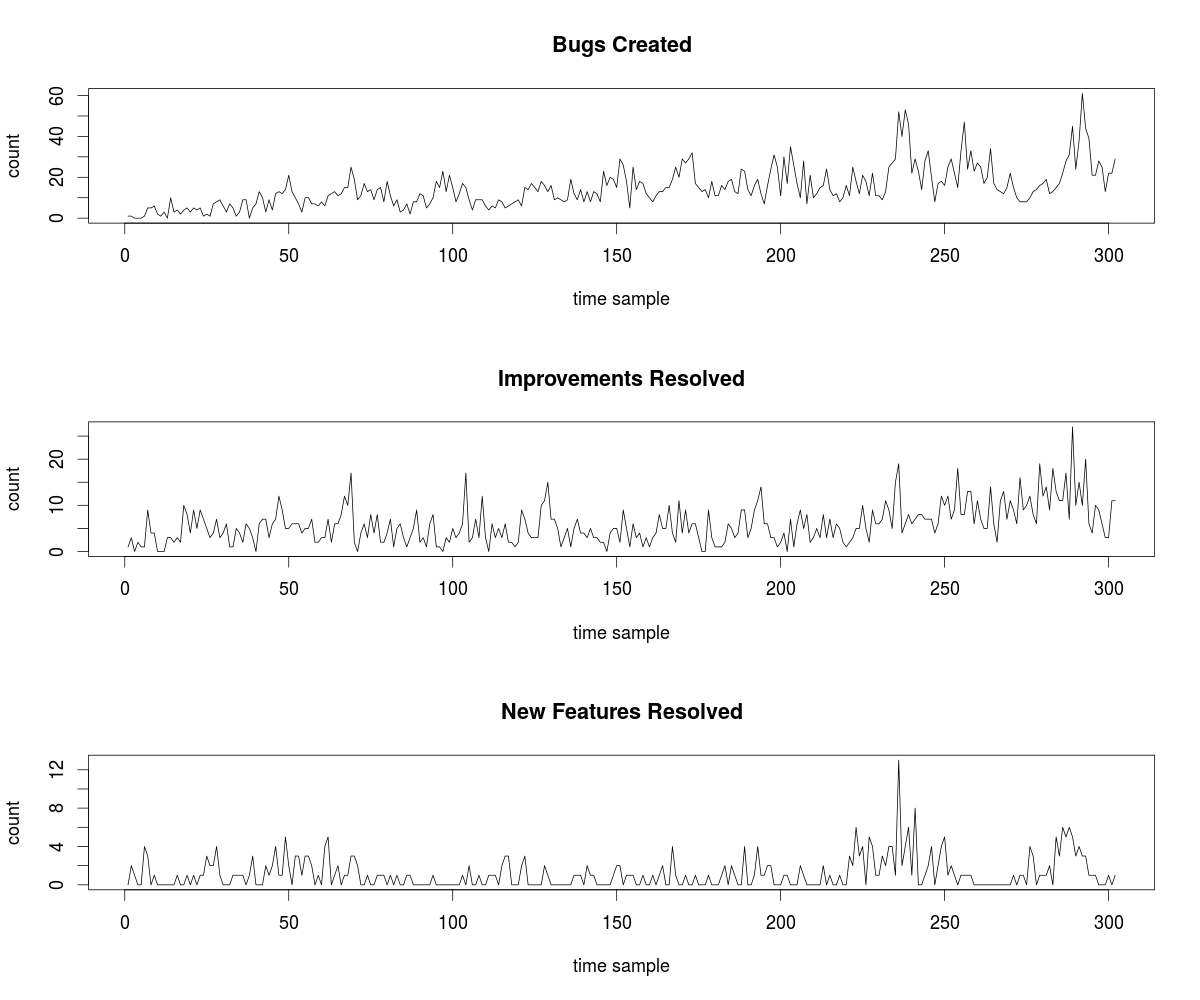
\includegraphics[width=\textwidth]{assets/time_series}
\caption[Time series data]{Time series data generated by sampling the \textit{MongoDB} dataset with a 7-day sample period.}
\label{fig:time_series}
\end{center}
\end{figure}

\section*{Stationarity Testing}

Before modeling, the time series were all checked for stationarity. The result of the ADF unit root and KPSS stationarity tests are listed in Table \ref{tab:stationarity_results}. The unit root tests showed less than $1\%$ significance for all time series. However, the stationarity test also showed low significance, meaning we have evidence to reject the hypothesis of stability. Since there is disagreement in the test results, the time series are differenced and the tests rerun.

\begin{table}[htbp]
  \centering
  \begin{tabular}{ c | r r | r r | r r }
      & \multicolumn{2}{|c|}{$Y_{bug}$} & \multicolumn{2}{|c|}{$Y_{imp}$} & \multicolumn{2}{|c}{$Y_{new}$} \\
    Statistic & value & signif. & value & signif. & value & signif. \\
    \hline
    ADF ($\tau_2$) & -5.0203 & $< 1\%$ & -7.4022 & $< 1\%$ & -7.8448 & $< 1\%$ \\
    ADF ($\phi_1$) & 12.6505 & $< 1\%$ & 27.4154 & $< 1\%$ & 30.7709 & $< 1\%$ \\
    KPSS & 2.8521 & $< 1\%$ & 2.0208 & $< 1\%$ & 0.5269 & $2.5-5\%$ \\
    \hline
  \end{tabular}
\caption[Stationarity test results]{Results of running the ADF unit root test and KPSS stationarity test on $Y_{bug}$, $Y_{imp}$, and $Y_{new}$. The tests are ran using an intercept-only regression model.}
\label{tab:stationarity_results}
\end{table}

After differencing we obtain the time series shown in figure \ref{fig:differenced_time_series}, which will be referred to as $Y_{\bigtriangledown bug}$, $Y_{\bigtriangledown imp}$, and $Y_{\bigtriangledown new}$. Now the result of the unit root and stationarity test (listed in Table \ref{tab:first_diff_stationarity_results}) both agree. That is, we can reject the hypothesis that a unit root (stochastic trend) is present at the $1\%$  significance level and we fail to reject the hypothesis of stationarity with greater than $10\%$ significance. Hence, the differenced time series will be used to move forward with modeling.

\begin{figure}[htbp]
\begin{center}
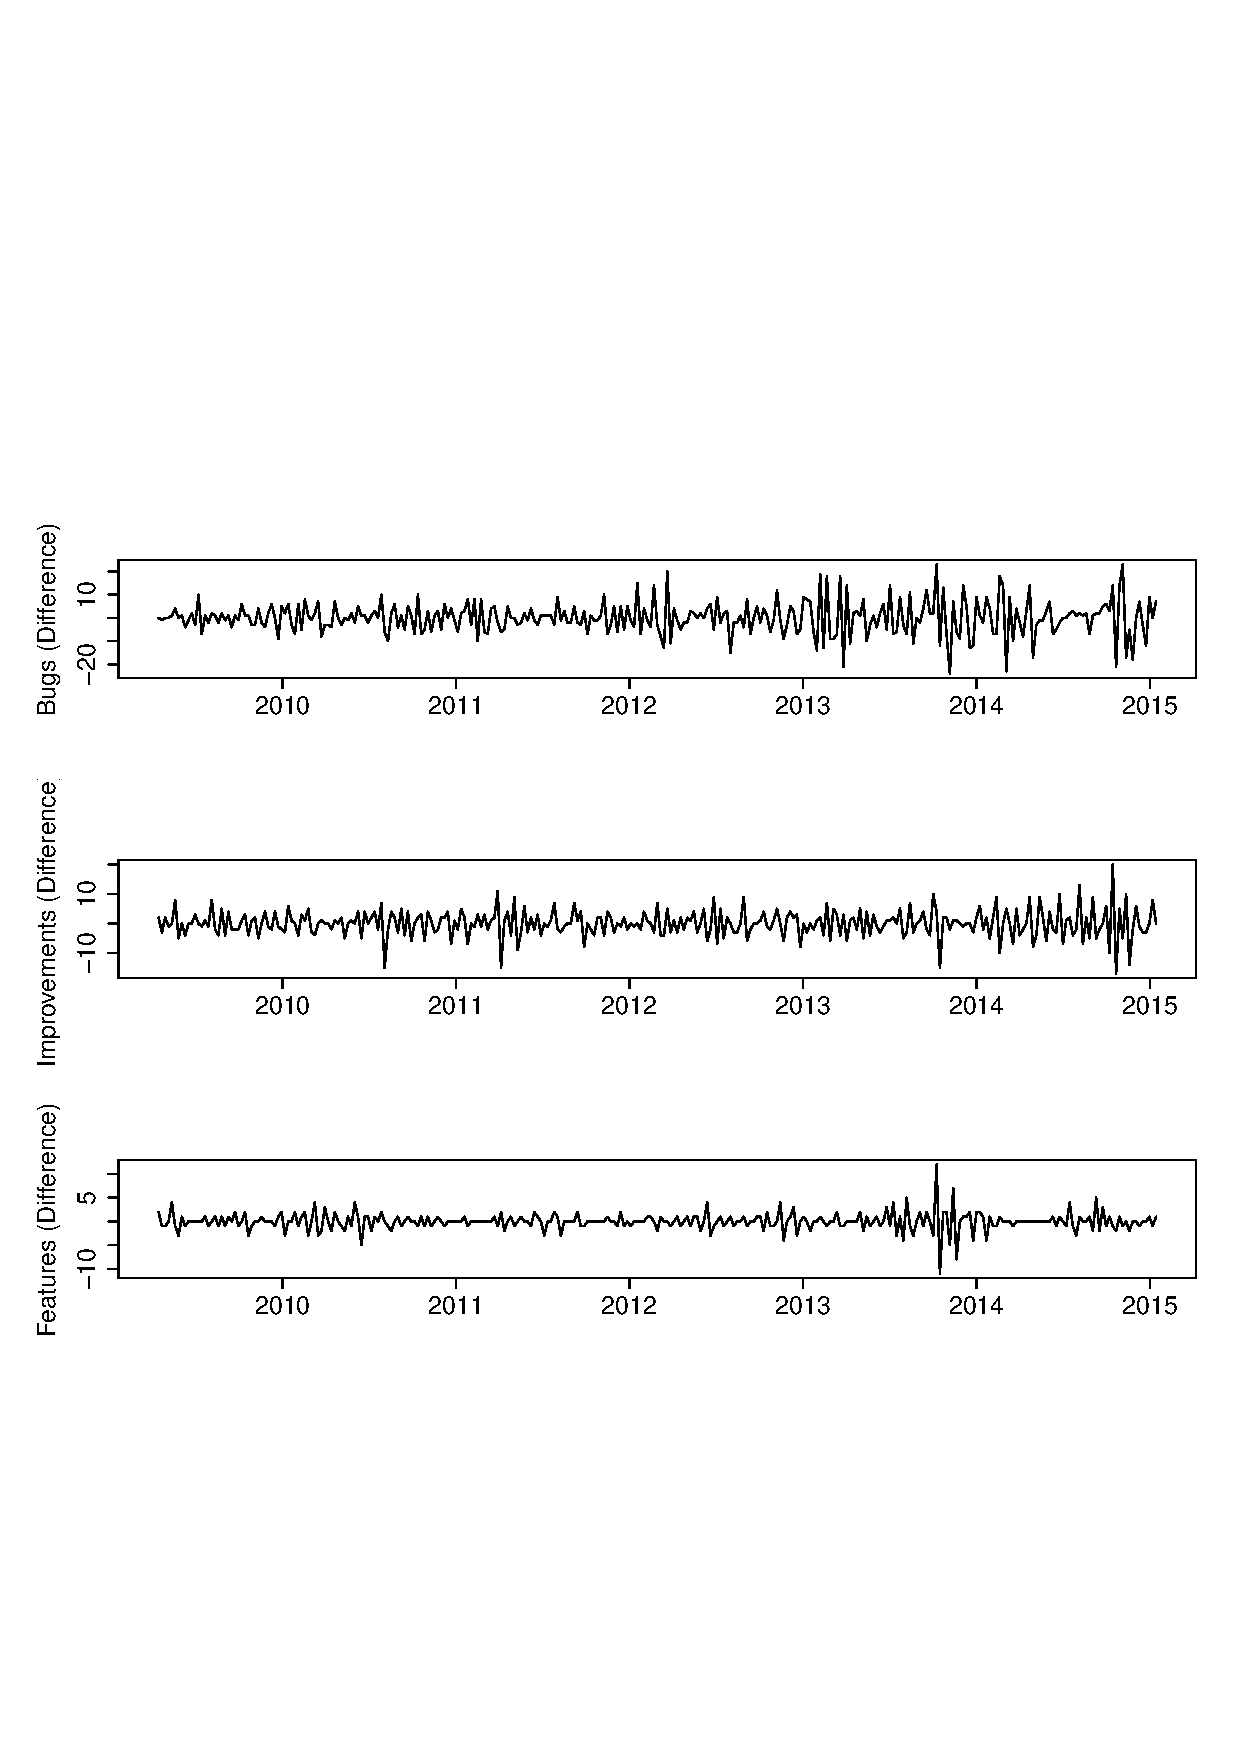
\includegraphics[width=\textwidth]{assets/time_series_diff}
\caption[Differenced time series]{Differenced time series data.}
\label{fig:differenced_time_series}
\end{center}
\end{figure}

\begin{table}[htbp]
  \centering
  \begin{tabular}{ c | r r | r r | r r }
      & \multicolumn{2}{|c|}{$Y_{\bigtriangledown bug}$} & \multicolumn{2}{|c|}{$Y_{\bigtriangledown imp}$} & \multicolumn{2}{|c}{$Y_{\bigtriangledown new}$} \\
    Statistic & value & signif. & value & signif. & value & signif. \\
    \hline
    ADF ($\tau_2$) & -17.6529 & $< 1\%$ & -20.4382 & $< 1\%$ & -21.8989 & $< 1\%$ \\
    ADF ($\phi_1$) & 155.8144 & $< 1\%$ & 208.8647 & $< 1\%$ & 239.7814 & $< 1\%$ \\
    KPSS & 0.0115 & $> 10\%$ & 0.0127 & $> 10\%$ & 0.0127 & $> 10\%$ \\
    \hline
  \end{tabular}
\caption[Stationary test results for differenced time series]{Results of running the ADF unit root test and KPSS stationarity test on the differenced time series}
\label{tab:first_diff_stationarity_results}
\end{table}

\section*{Time Windowing}
A 78-week time window (approximately 18 months) was established to restrict model scope. Three of these windowed periods, non-overlapping, were kept for modeling. Since the data is being differenced, the first sample (week) is skipped. These windowed periods are denoted $W_{2-79}$, $W_{80-157}$, and $W_{158-235}$.

\section*{Time Series Model}

The modeling methodology was applied to the time series data, to produce a VARX model for each windowed period. The $Y_{\bigtriangledown new}$ and $Y_{\bigtriangledown imp}$ time series were both considered exogenous, so that their hypothetical future values alone could be used to make defect predictions.

\section*{Model Specification \& Estimation}

By selecting $K_{min} = 4$, a maximum model order is obtained by
\begin{equation}
p_{max} = \left \lfloor \frac{78}{(3)(4)} \right \rfloor = \lfloor 6.5 \rfloor = 6
\end{equation}

So models of order $1$ through $p_{max}=6$ were estimated for later diagnostic checking.

\section*{Model Diagnostic Checking}

Candidate models were tested for stability and inadequacy. A $5\%$ significance level was used in the Ljung-Box test. The results for each windowed period are shown in table \ref{tab:diagnostic_results}. All model orders were stable for all windowed periods. Several model orders were found to be inadequate by the Ljung-Box test: orders 1-2 for period $W_{2-79}$, and order 5 for period $W_{158-235}$.

\begin{table}[htbp]
  \centering
  \begin{tabular}{ c | r r | r r | r r }
      & \multicolumn{2}{|c|}{$W_{2-79}$} & \multicolumn{2}{|c|}{$W_{80-157}$} & \multicolumn{2}{|c}{$W_{158-235}$} \\
    Model order & stable & p-value & stable & p-value & stable & p-value \\
    \hline
    1 & Yes & 0.009061 & Yes & 0.4478 & Yes & 0.09453 \\
    2 & Yes & 0.01401 & Yes & 0.5866 & Yes & 0.1255 \\
    3 & Yes & 0.2052 & Yes & 0.6470 & Yes & 0.1753 \\
    4 & Yes & 0.1288 & Yes & 0.7596 & Yes & 0.09363 \\ 
    5 & Yes & 0.3363 & Yes & 0.6133 & Yes & 0.04656 \\
    6 & Yes & 0.2818 & Yes & 0.3838 & Yes & 0.05703 \\
    \hline
  \end{tabular}
\caption[Diagnostic test results]{Results of running stability and Ljung-Box test on each windowed period.}
\label{tab:diagnostic_results}
\end{table}

\section*{Model Selection}
Models that were not rejected for instability or inadequacy were then compared and the best for each windowed period was selected by AIC selection criterion. The results of selection are the bolded values shown in Table \ref{tab:selection_results}. The fit for each of these models is demonstrated by plotting one-step predictions along with actual values, as shown for each model in figure \ref{fig:one_step_predictions}. The fit for each appears to track well with many of the significant changes in the time series.

\begin{table}[htbp]
  \centering
  \begin{tabular}{ c | r | r | r }
    ~ & \multicolumn{3}{|c}{AIC score} \\
    Model order & $W_{2-79}$ & $W_{80-157}$ & $W_{158-235}$ \\
    \hline
    1 & N/A & 429.8 & 477.9 \\
    2 & N/A & 439.3 & 482.4 \\
    3 & 400.8 & 440.9 & 489.7 \\
    4 & 400.3 & 450.2 & 499.9 \\ 
    5 & 404.0 & 456.7 & N/A \\
    6 & 414.9 & 461.7 & 508.8 \\
    \hline
  \end{tabular}
\caption[Model selection results]{Results of model selection, using AIC score to compare models of different order.}
\label{tab:selection_results}
\end{table}

\begin{figure}[htbp]
\centering
\subfloat[Windowed period $W_{2-79}$]{
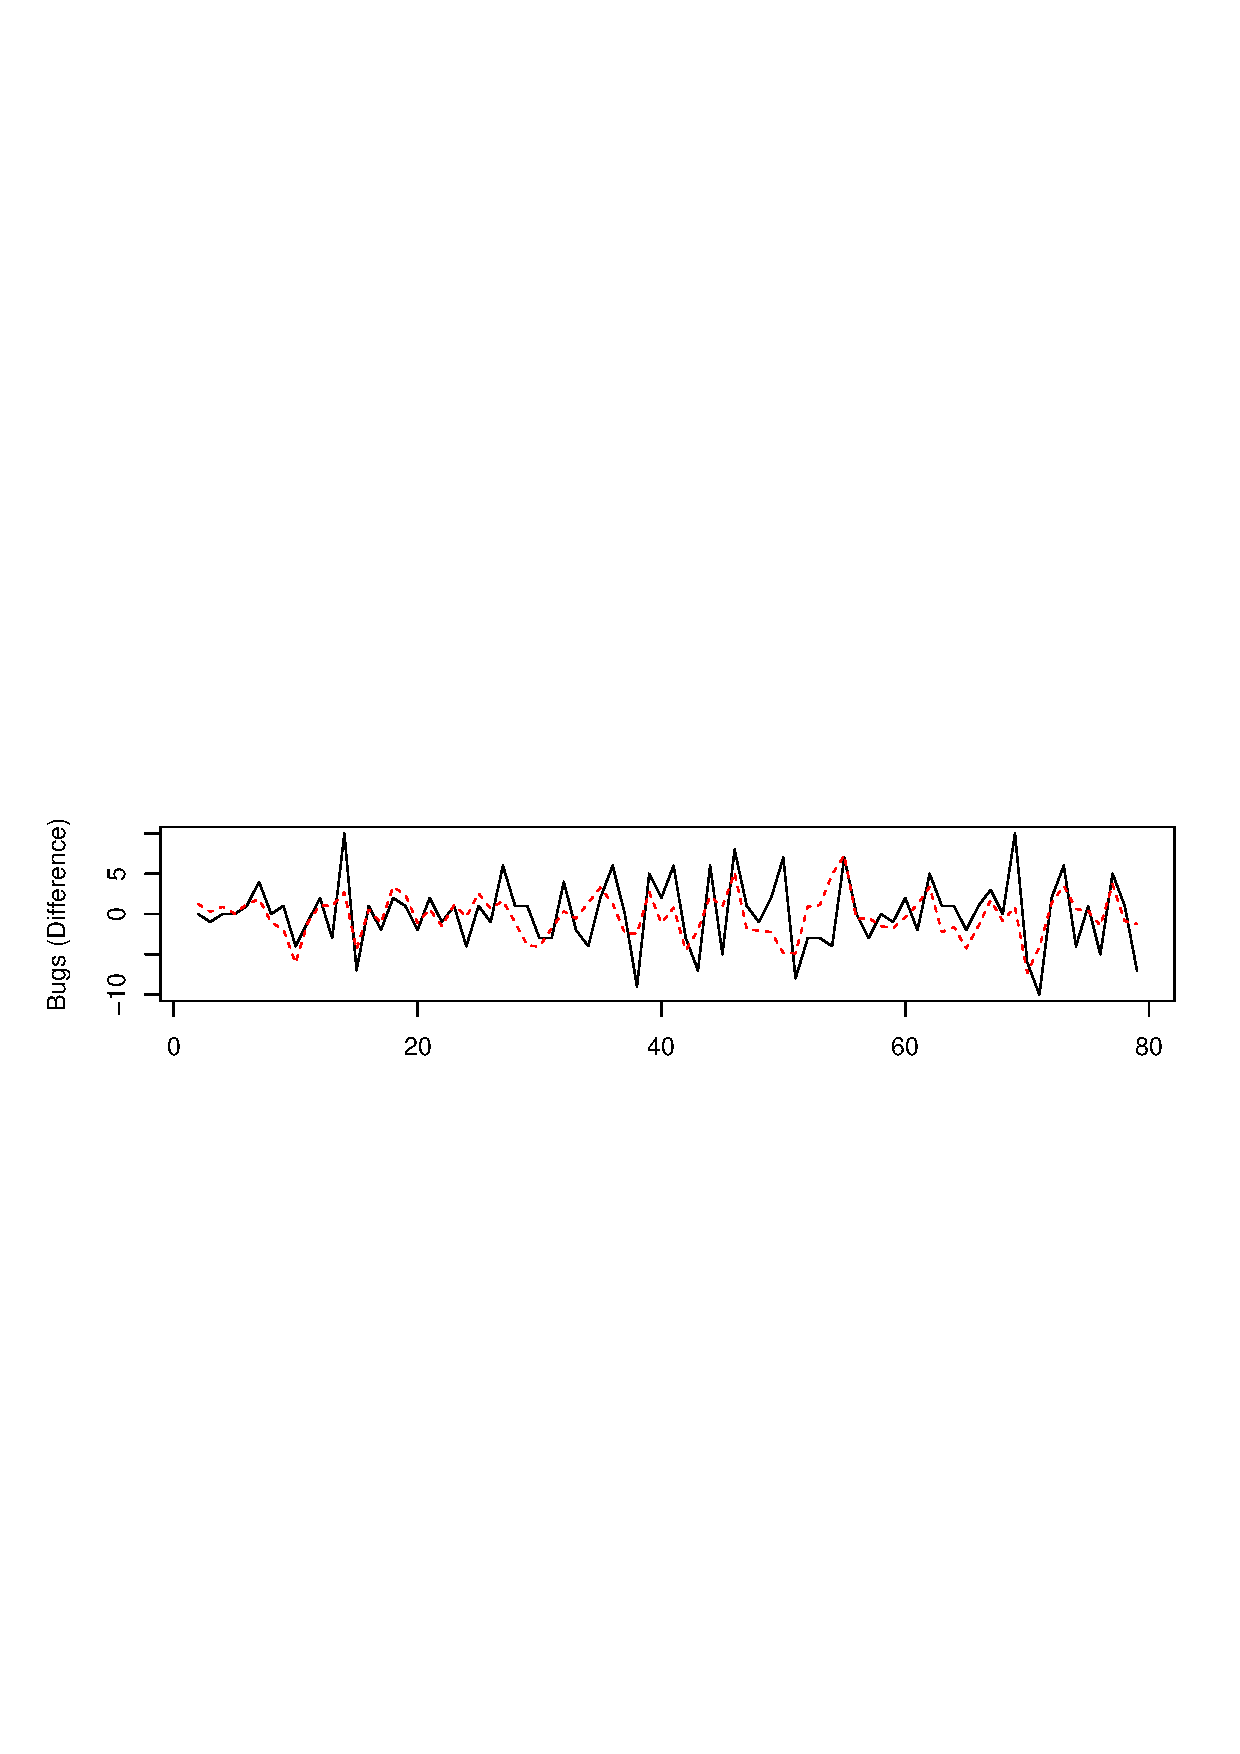
\includegraphics[width=\textwidth]{assets/one-step_predictions_2-79}
}\\
\subfloat[Windowed period $W_{80-157}$]{
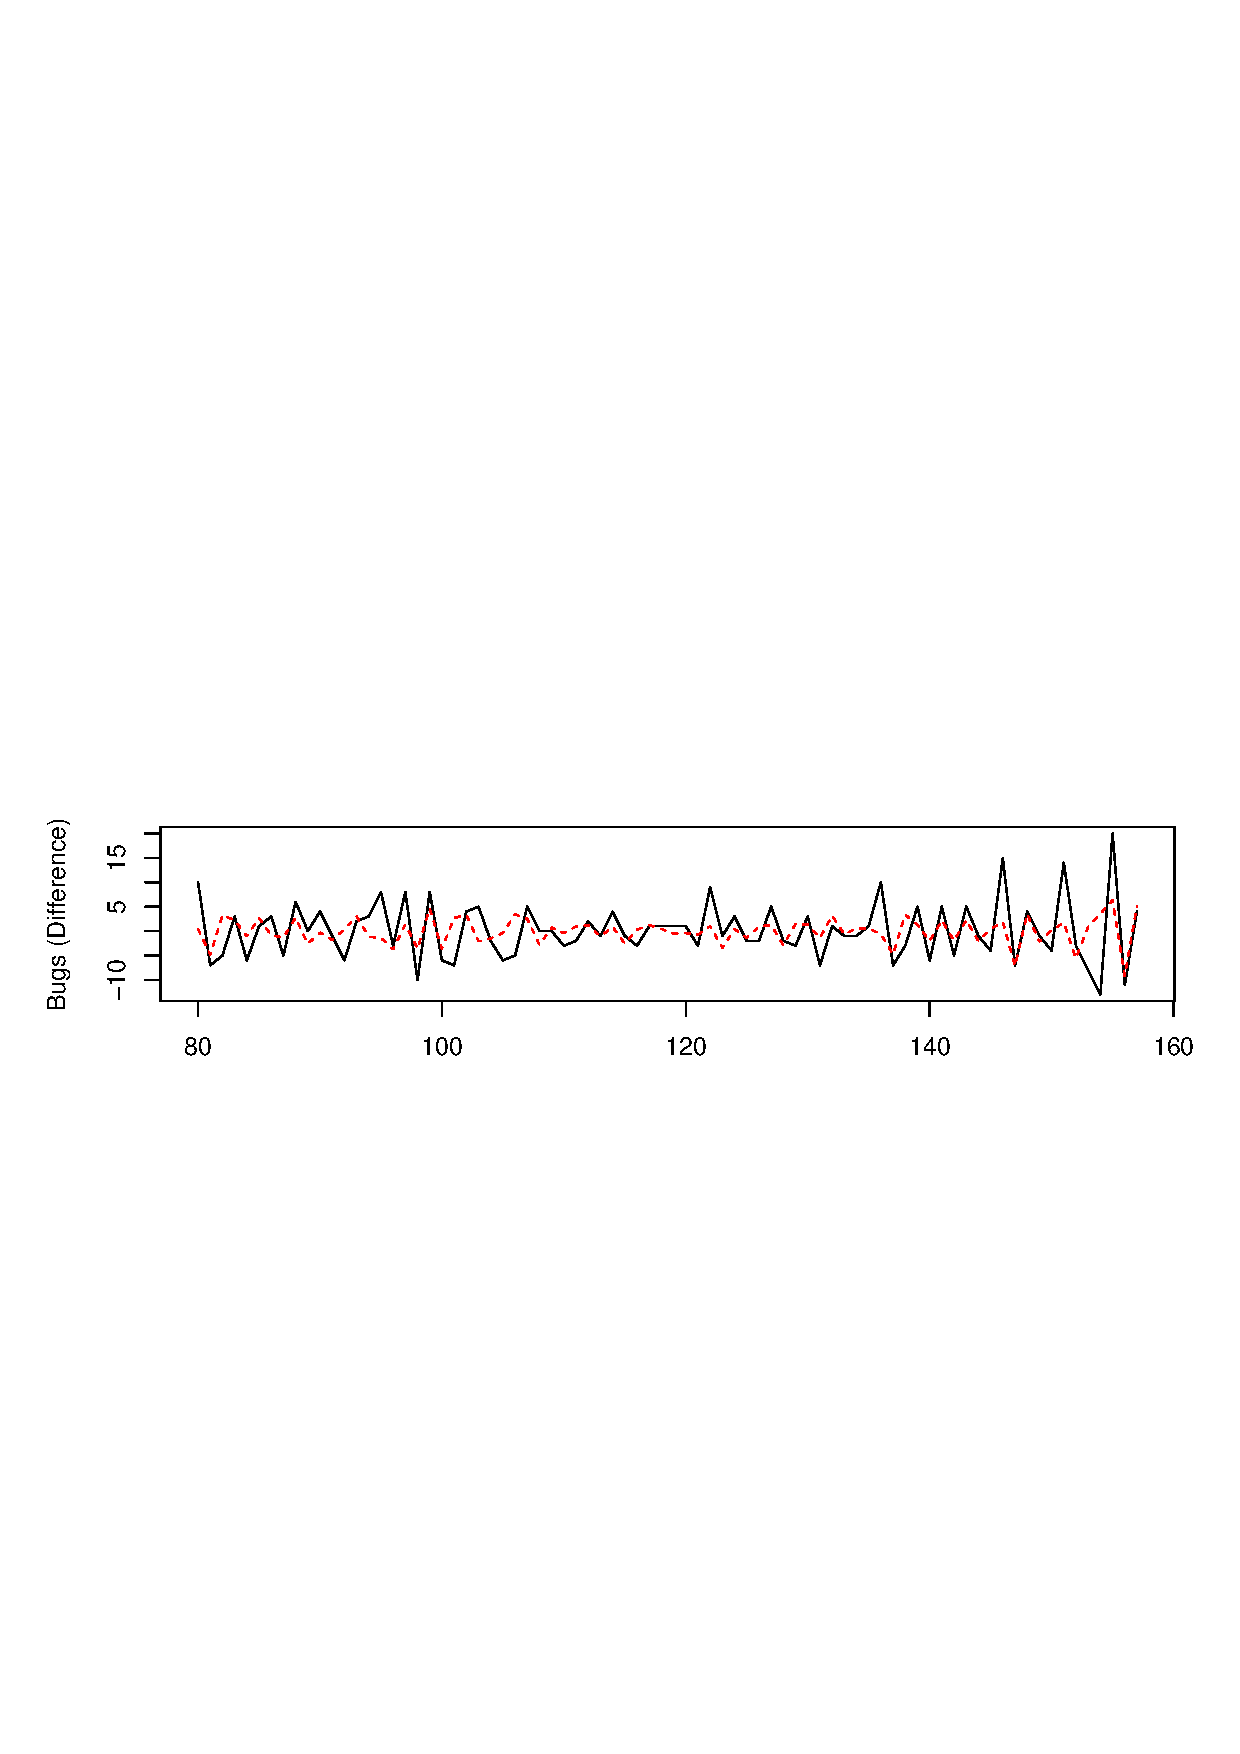
\includegraphics[width=\textwidth]{assets/one-step_predictions_80-157}
}\\
\subfloat[Windowed period $W_{158-235}$]{
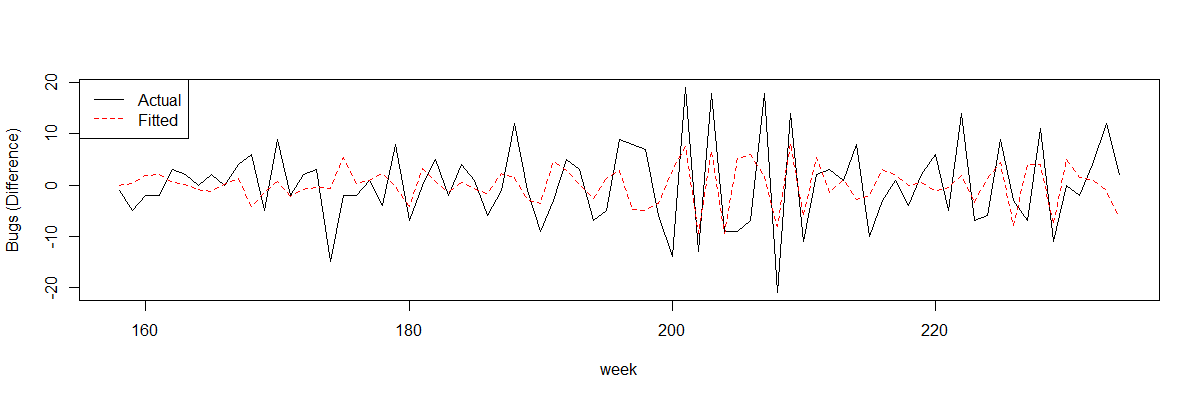
\includegraphics[width=\textwidth]{assets/one-step_predictions_158-235}
}%
\caption[One-step predictions]{One-step predictions vs actual values, for each model selected by AIC score.}
\label{fig:one_step_predictions}
\end{figure}


\section*{Forecasting}

The model selected for each windowed period was used to forecast the number of defects in the next sample after the end of the window. The input for making these predictions was the number of improvements and features that were expected to be resolved. The input values were converted to differences, since the underlying model was formed using differenced data. Differencing was then removed to provide the predicted number of future defects.

Table \ref{tab:forecasting_results} shows the resulting single-step, out-of-sample defect prediction data for the first time window, $W_{2-79}$, including the upper and lower bounds of the confidence intervals. The actual number of improvements, features, and bugs in the prediction sample period was 4, 0, and 18, respectively. Notice that the actual number of bugs, 18, is outside of the 90\% confidence interval, which spans from 6.4 to 13.79 (see the bold outlined row in Table \ref{tab:forecasting_results}). On the other hand, the actual number of future defects in the next window, $W_{80−157}$, was 17. This was inside the 90\% confidence interval, which spans from 13.38 to 18.00.

\begin{table}[htbp]
  \centering
  \begin{tabular}{ c | c | c | c | c | c | c }
    Improvements & Features & 90\% low & 75\% low & Mean & 75\% high & 90\% high \\
    \hline
2 & 0 & 5.61 & 6.72 & 9.31 & 11.89 & 13.00 \\
2 & 1 & 5.54 & 6.66 & 9.24 & 11.82 & 12.93 \\
2 & 2 & 5.48 & 6.59 & 9.17 & 11.75 & 12.86 \\
2 & 3 & 5.41 & 6.52 & 9.1 & 11.69 & 12.8 \\
4 & 0 & 6.4 & 7.51 & 10.09 & 12.68 & 13.79 \\
4 & 1 & 6.33 & 7.44 & 10.03 & 12.61 & 13.72 \\
4 & 2 & 6.27 & 7.38 & 9.96 & 12.54 & 13.65 \\
4 & 3 & 6.2 & 7.31 & 9.89 & 12.48 & 13.59 \\
    \hline
  \end{tabular}
\caption[Forecasting results]{Forecasting at the end of the first time window, $W_{2-79}$. Future output values are predicted for a number of hypothetical input values.}
\label{tab:forecasting_results}
\end{table}

To gauge how well prediction will work in general, a sliding 78-week window was applied. The sliding window started at the first sample period, and was shifted by one sample period after modeling. Only the actual number of improvements and features were used in this forecasting. The resulting distribution of errors between the mean forecasted bugs and the actual number of bugs is shown as a histogram in Figure \ref{fig:forecast_errors}. Note that the histogram appears to be normally distributed.  The actual number of bugs was inside the 90\% confidence interval for 23.87\% of the sliding window ranges.

\begin{figure}[htbp]
\centering
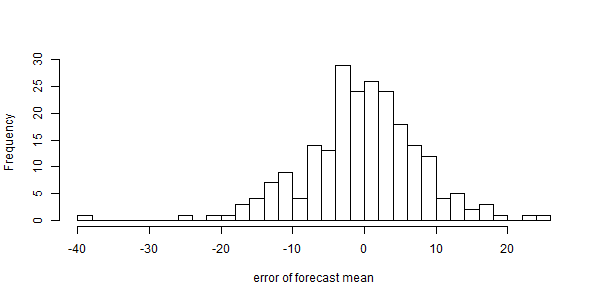
\includegraphics[width=\textwidth]{assets/forecast_errors}
\caption[Forecast errors]{Histogram of forecast mean errors obtained using a 78-week sliding window.}
\label{fig:forecast_errors}
\end{figure}

\chapter{Conclusions and Future Work}
\label{sec:conclusions}
The VARX modeling methodology was successfully applied to the time series data collected from the \textit{MongoDB} project. A model was created for each of three time windows and then used to make defect predictions for a range of hypothetical values for the number of improvements and features. Also, a picture of the prediction performance was obtained by applying the approach with a sliding window. This resulted in a normally distributed error between the mean forecasted and actual number of bugs. A low proportion (23.87\%) of the sliding window ranges included the actual number of bugs using a 90\% confidence interval. These results indicate that the VARX model had a low prediction accuracy for the actual number of defects in the MongoDB dataset.

Having applied the VARX time series model to one project dataset, a next step is to apply the methodology to other software project data sets, such as \textit{Eclipse} or \textit{Mozilla}, to better determine the applicability of the modeling approach. The estimated time to complete this additional work is one month. 

%The time estimated to complete this additional work is summarized in the timeline shown in Table \ref{tab:timeline}.
%
%\begin{table}[h]
%\centering
%\begin{tabular}{ p{2.5in} l l}
%\hline
%Task & Date \\
%\hline
%Form committee & Mar 9-13 \\
%Present proposal & Mar 18 \\
%Respond to committee feedback & Mar 18 - Apr 8 \\
%Apply models for release planning & Apr 1-15 \\
%Repeat on two other SW projects & Apr 15 - May 6 \\
%\hline
%\end{tabular}
%\caption[Timeline for proposed work]{Timeline for proposed work}
%\label{tab:timeline}
%\end{table}


%%\appendix
%%\chapter{Software Requirements}
%%\label{sw_reqs}
%%The software developed so far has been used for data collection and analysis. The scripts used can be run on any platform that supports Python and R. Besides this basic requirement, here are the other dependencies:
%%\paragraph{Python dependencies:}
%%\begin{itemize}
%%\item
%%docopt: for defining command-line interfaces and parsers. See the \href{https://github.com/docopt/docopt}{GitHub page} for installation instructions.
%%\item
%%BeatifulSoup: for processing XML files. See the \href{http://www.crummy.com/software/BeautifulSoup}{support page} for installation instructions.
%%\end{itemize}
%%
%%\paragraph{R dependencies:}
%%\begin{itemize}
%%%\item
%%%devtools: adds github\_install function. Install by running ``\verb|install.packages("devtools")|" on the R command line.
%%%\item{docopt: for defining command-line interfaces and parsers. See the \href{https://github.com/edwindj/docopt.R}{GitHub page} for installation instructions.}
%%\end{itemize}


\bibliography{references}
\bibliographystyle{abbrv}

\end{document}